%%%%%%%%%%%%%%%%%%%%%%%%%%%%%%%%%%%%

\section{確率変数}

%%%%%%%%%%%%%%%%%%%%%%%%%%%%%%%%%%%%

\begin{frame}
\frametitle{確率変数}

\begin{itemize}

\item \hl{確率変数}とは、確率的事象の結果に依存する数値量のことである
\begin{itemize}
\item 確率変数を表すために $X$ のような大文字を使う
\item 確率変数の値は小文字、ここでは $x$ で表す
\item 例：$P(X = x)$
\end{itemize}

\item 確率変数には2種類ある：
\begin{itemize}
\item \hl{離散確率変数}はしばしば整数値のみをとる
\begin{itemize}
\item 例：履修単位数、今学期と前学期の履修単位数の差
\end{itemize}
\item \hl{連続確率変数}は実数（小数）値をとる
\begin{itemize}
\item 例：今学期の教科書代、今学期と前学期の教科書代の差
\end{itemize}
\end{itemize}

\end{itemize}

\end{frame}

%%%%%%%%%%%%%%%%%%%%%%%%%%%%%%%%%%%%

\subsection{期待値}

%%%%%%%%%%%%%%%%%%%%%%%%%%%%%%%%%%%%

\begin{frame}
\frametitle{期待値}

\begin{itemize}

\item 確率変数の平均的な結果にしばしば関心がある。

\item これを\hl{期待値}（平均）と呼び、可能な結果の加重平均である
\formula{\[\mu = E(X) = \sum_{i = 1}^k x_i ~ P(X = x_i)\]}

\end{itemize}

\end{frame}

%%%%%%%%%%%%%%%%%%%%%%%%%%%%%%%%%%%%

\begin{frame}
\frametitle{離散確率変数の期待値}

\dq{カードゲームで、ハートを引いたら1ドル、エース（ハートのエースを含む）を引いたら5ドル、スペードのキングを引いたら10ドル、それ以外のカードを引いたら何も得られない。勝利金の確率モデルを書き、期待される勝利金を計算しなさい。}

\begin{center}
\renewcommand{\arraystretch}{1.5}
\begin{tabular}{l | c | c | c }
事象		& $X$ 		& $P(X)$        		& $X ~ P(X)$ \\
\hline
ハート（エース以外）	& $1$		& $\frac{12}{52}$	& $\frac{12}{52}$ \\
エース			& $5$		& $\frac{4}{52}$	& $\frac{20}{52}$ \\
スペードのキング	& $10$		& $\frac{1}{52}$	& $\frac{10}{52}$ \\
その他		& $0$		& $\frac{35}{52}$	& $0$ \\
\hline
合計			&			&				& $E(X) = \frac{42}{52} \approx 0.81$
\end{tabular}

\end{center}

\end{frame}

%%%%%%%%%%%%%%%%%%%%%%%%%%%%%%%%%%%%

\begin{frame}
\frametitle{離散確率変数の期待値（続き）}

以下はこのゲームの勝利金の確率分布を視覚的に表したものである：

\begin{center}
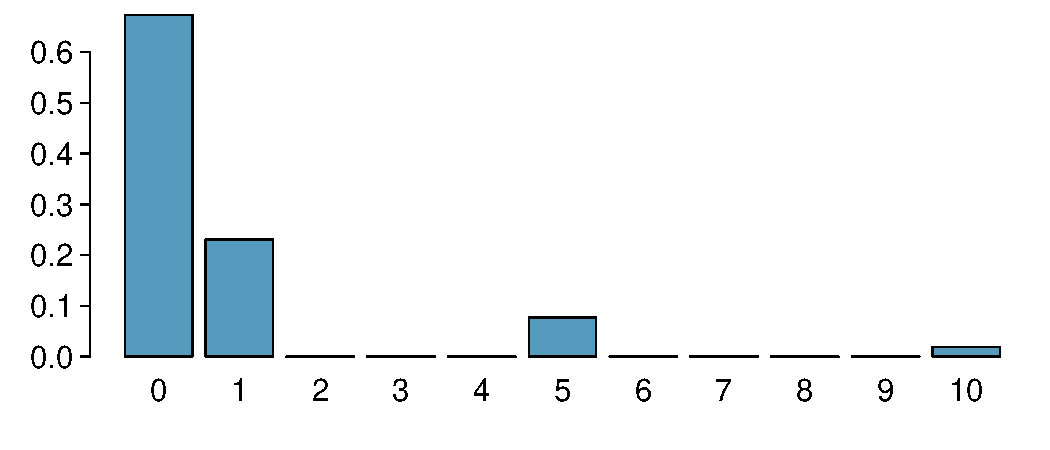
\includegraphics[width=0.8\textwidth]{3-4_random_variables/figures/card_game/card_game}
\end{center}

\end{frame}

%%%%%%%%%%%%%%%%%%%%%%%%%%%%%%%%%%%%

\subsection{確率変数の変動性}

%%%%%%%%%%%%%%%%%%%%%%%%%%%%%%%%%%%%

\begin{frame}
\frametitle{変動性}

確率変数の値の変動性にもしばしば関心がある。

\formula{
\[ \sigma^2 = Var(X) = \sum_{i = 1}^k (x_i - E(X))^2 P(X = x_i) \]
\[ \sigma = SD(X) = \sqrt{Var(X)} \]
}

\end{frame}

%%%%%%%%%%%%%%%%%%%%%%%%%%%%%%%%%%%%

\begin{frame}[shrink=15]
\frametitle{離散確率変数の変動性}

\dq{先のカードゲームの例で、ゲームごとに勝利金がどのくらい変動すると予想されるか？}

\vspace{2mm}
{\footnotesize
\begin{center}
\renewcommand{\arraystretch}{2}
\begin{tabular}{c | c | c | l | p{4cm}}
$X$ & $P(X)$         & $X ~ P(X)$      & \multicolumn{1}{c|}{$(X - E(X))^2$}  & \multicolumn{1}{c}{$P(X) ~ (X - E(X))^2$}  \\
\hline
1 & $\frac{12}{52}$  & $1 \times \frac{12}{52} = \frac{12}{52}$ & $(1 - 0.81)^2 = 0.0361$ &  $\frac{12}{52} \times 0.0361 = 0.0083$ \\
\hline
5 & $\frac{4}{52}$   & $5 \times \frac{4}{52} = \frac{20}{52}$ & $(5 - 0.81)^2 = 17.5561$  & $\frac{4}{52} \times 17.5561 = 1.3505$ \\
\hline
10  & $\frac{1}{52}$ & $10 \times \frac{1}{52} = \frac{10}{52}$  & $(10 - 0.81)^2 = 84.4561$   & $\frac{1}{52} \times 84.0889 = 1.6242$ \\
\hline
0 & $\frac{35}{52}$  & $0 \times \frac{35}{52} = 0$  & $(0 - 0.81)^2 = 0.6561$ & $\frac{35}{52} \times 0.6561 = 0.4416$ \\
\hline
  &       & $E(X) = 0.81$ & & \soln{$V(X) = 3.4246$} \\
 &       &                                                         & & \soln{$SD(X) = \sqrt{3.4246} = 1.85$} \\
\end{tabular}
\end{center}
}
\end{frame}

%%%%%%%%%%%%%%%%%%%%%%%%%%%%%%%%%%%%

\subsection{確率変数の線形結合}

%%%%%%%%%%%%%%%%%%%%%%%%%%%%%%%%%%%%

\begin{frame}
\frametitle{線形結合}

\begin{itemize}

\item 確率変数 $X$ と $Y$ の\hl{線形結合}は次のように表される

\[ aX + bY \]

ここで $a$ と $b$ はある固定された数である。

\item 確率変数の線形結合の平均値は次のように計算される
\formula{\[ E(aX + bY) = a \times E(X) + b \times E(Y) \]}

\end{itemize}

\end{frame}

%%%%%%%%%%%%%%%%%%%%%%%%%%%%%%%%%%%%

\begin{frame}
\frametitle{線形結合の期待値の計算}

\dq{統計学の宿題問題1つには平均10分、化学の宿題問題1つには平均15分かかる。今週は統計学の宿題5問と化学の宿題4問が出された。今週の統計学と化学の宿題に費やすと予想される合計時間は何か？}

\soln{
\begin{align*}
&E(S + S + S + S + S + C + C + C + C)  \\
&= 5 \times E(S) + 4 \times E(C) \\
&= 5 \times 10 + 4 \times 15 \\
&= 50 + 60 \\
&= 110~\text{分}
\end{align*}
}

\end{frame}

%%%%%%%%%%%%%%%%%%%%%%%%%%%%%%%%%%%%

\subsection{確率変数の線形結合の変動性}

%%%%%%%%%%%%%%%%%%%%%%%%%%%%%%%%%%%%

\begin{frame}
\frametitle{線形結合}

\begin{itemize}

\item 2つの独立な確率変数の線形結合の変動性は次のように計算される

\formula{\[ V(aX + bY) = a^2 \times V(X) + b^2 \times V(Y) \]}

\item 線形結合の標準偏差は分散の平方根である。

\end{itemize}

\vfill

\Note{確率変数が独立でない場合、分散の計算はやや複雑になり、本講義の範囲を超える。}

\end{frame}

%%%%%%%%%%%%%%%%%%%%%%%%%%%%%%%%%%%%

\begin{frame}
\frametitle{線形結合の分散の計算}

\dq{統計学の宿題問題1つにかかる時間の標準偏差は1.5分、化学の宿題問題1つには2分である。統計学の宿題5問と化学の宿題4問が出された今週に統計学と物理学の宿題に費やすと予想される時間の標準偏差は何か？各問題にかかる時間は互いに独立であると仮定する。}

\soln{
\begin{align*}
&V(S + S + S + S + S + C + C + C + C)  \\
&= V(S) + V(S) + V(S) + V(S) + V(S)  \\
&+ V(C) + V(C) + V(C) + V(C) \\
&= 5 \times V(S) + 4 \times V(C) \\
&= 5 \times 1.5^2 + 4 \times 2^2 \\
&= 27.25
\end{align*}
}

\end{frame}

%%%%%%%%%%%%%%%%%%%%%%%%%%%%%%%%%%%%

\subsection{まとめ}

%%%%%%%%%%%%%%%%%%%%%%%%%%%%%%%%%%%%

\begin{frame}[shrink=20]
\frametitle{練習問題}

\pq{カジノゲームのプレイに5ドルかかる。最初に引いたカードが赤であれば、2枚目のカードを（非復元で）引ける。2枚目がクラブのエースであれば500ドルを獲得する。そうでなければ、何も得られず（5ドルを失う）。このゲームをプレイしたときの期待利益/損失は何か？ {\small 覚えておこう：利益/損失 = 賞金 - コスト。}}

\begin{multicols}{2}
\begin{enumerate}[(a)]
\item 5セントの利益
\solnMult{10セントの損失}
\item 25セントの損失
\item 30セントの損失
\end{enumerate}
\end{multicols}

\soln{
{\small
\renewcommand\arraystretch{1.25}
\begin{tabular}{l c c c r}
事象				& 賞金	& 利益: $X$	& $P(X)$	& $ X \times P(X)$	\\
\hline
\orange{赤}, {A}{$\clubsuit$}		& 500		& 500 - 5 = 495	& $\frac{26}{52} \times \frac{1}{51} = 	0.0098$ & 	 $495 \times 0.0098 = 4.851$ \\
その他	& 0 			& 0 - 5 = -5	& $1 - 0.0098 = 0.9902$ & $-5 \times 0.9902 = -4.951$ \\
\hline
					&			&			& 			& $E(X) = -0.1$
\end{tabular}
}
}

\end{frame}

%%%%%%%%%%%%%%%%%%%%%%%%%%%%%%%%%%%%

\begin{frame}[shrink=10]
\frametitle{公正なゲーム}

\hl{公正な}ゲームとは、コストが期待される賞金額と同じ、すなわち期待利益が0のゲームである。

$\:$

\dq{ラスベガスのカジノゲームは、期待される賞金額より多くかかると思うか、少なくかかると思うか？}

\soln{
\begin{columns}[c]
\column{0.6\textwidth}
もしそれらのゲームが期待される賞金額より少なければ、カジノは平均的に損をしていることになり、以下のようなものに費用を払えなくなる：
\column{0.4\textwidth}
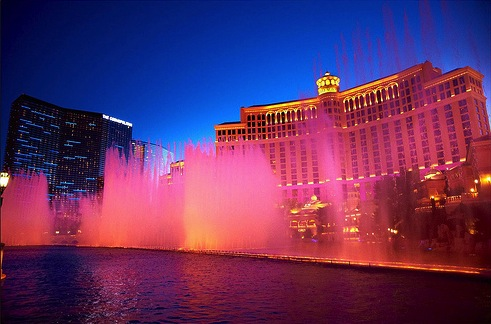
\includegraphics[width=\textwidth]{3-4_random_variables/figures/bellagio.jpg}
\end{columns}
\ct{Image by Moyan\_Brenn on Flickr \webURL{http://www.flickr.com/photos/aigle\_dore/5951714693}.}
}


\end{frame}

%%%%%%%%%%%%%%%%%%%%%%%%%%%%%%%%%%%%%

\begin{frame}
\frametitle{確率変数の簡略化}

確率変数は通常の代数変数とは異なる振る舞いをする：
\[ X + X \ne 2X \]

{\small
\twocol{0.45}{0.45}
{
\begin{align*}
E(X + X) &= E(X) + E(X) \\
&= 2 E(X) \\
&~  \\
E(2X) &= 2 E(X) \\
&~
\end{align*}
}
{
\begin{align*}
Var(X + X) &= Var(X) + Var(X)~{\scriptsize \text{（独立を仮定）}} \\
&= 2~Var(X) \\
&~  \\
Var(2X) &= 2^2~Var(X) \\
&= 4~Var(X)
\end{align*}
}
}

\vspace{3mm}

\mathhl{E(X + X)  = E(2X)} だが、\mathhl{Var(X + X) \ne Var(2X)} である。

\end{frame}

%%%%%%%%%%%%%%%%%%%%%%%%%%%%%%%%%%%%%

\begin{frame}[shrink=25]
\frametitle{足し算か掛け算か？}

\dq{ある会社のフリートに5台のリンカーン・タウンカーがある。過去のデータによると、各車の年間メンテナンスコストは平均2,154ドル、標準偏差は132ドルである。このフリートの年間総メンテナンスコストの平均と標準偏差は何か？}

1台の車が年間メンテナンスコストの5倍 $(5X)$ ではなく、それぞれ同じ年間メンテナンスコストを持つ5台の車 $(X_1 + X_2 + X_3 + X_4 + X_5)$ であることに注意する。

{\small
\begin{eqnarray*}
E(X_1 + X_2 + X_3 + X_4 + X_5) &=& E(X_1) + E(X_2) + E(X_3) + E(X_4) + E(X_5) \\
&=& 5 \times E(X) = 5 \times 2,154 = \$ 10,770 \\
Var(X_1 + X_2 + X_3 + X_4 + X_5) &=& Var(X_1) + Var(X_2) + Var(X_3) + Var(X_4) + Var(X_5) \\
&=& 5 \times V(X) = 5 \times 132^2 = \$ 87,120 \\
SD(X_1 + X_2 + X_3 + X_4 + X_5) &=& \sqrt{87,120} =  295.16
\end{eqnarray*}
}

\end{frame}

%%%%%%%%%%%%%%%%%%%%%%%%%%%%%%%%%%%%
